\documentclass[english]{SPFShortReport}
\usepackage{subfigure}
\usepackage{spfFigures}
\usepackage{longtable}
\usepackage{url}
\usepackage{gensymb}
\usepackage[yyyymmdd,hhmmss]{datetime}
\reportName{Python calculation for heat pump SIN-14TU}
\reportSubName{Parametric Heat Pump calculation} 
\reportDate{\today \hspace{0.1cm} at: \currenttime \hspace{0.1cm} h} 
\author{Dani Carbonell}
\address{dani.carbonell@solarenergy.ch}
\begin{document}
\begin{table}[!ht]
\begin{small}
\caption{Fitted coefficients for the heat pump.}
\begin{center}
\resizebox{12cm}{!} 
{
\begin{tabular}{l | c c } 
\hline
\hline
Coefficient &Description & \\ 
 & &$[kW]$\\ 
\hline
$PQ_{1}$ & \emph{$1^{st}$ condenser polynomial coefficient}  & 1.3258e+01    \\ 
$PQ_{2}$ & \emph{$2^{st}$ condenser polynomial coefficient}  & 1.5673e+02    \\ 
$PQ_{3}$ & \emph{$3^{st}$ condenser polynomial coefficient}  & 3.5853e+01    \\ 
$PQ_{4}$ & \emph{$4^{st}$ condenser polynomial coefficient}  & -2.6116e+02    \\ 
$PQ_{5}$ & \emph{$5^{st}$ condenser polynomial coefficient}  & 2.0242e+01    \\ 
$PQ_{6}$ & \emph{$6^{st}$ condenser polynomial coefficient}  & -1.8200e+02    \\ 
\hline
$PCOP_{1}$ & \emph{$1^{st}$ COP polynomial coefficient}  & 7.4744e+00    \\ 
$PCOP_{2}$ & \emph{$2^{st}$ COP polynomial coefficient}  & 8.2635e+01    \\ 
$PCOP_{3}$ & \emph{$3^{st}$ COP polynomial coefficient}  & -9.7922e+00    \\ 
$PCOP_{4}$ & \emph{$4^{st}$ COP polynomial coefficient}  & -3.2890e+02    \\ 
$PCOP_{5}$ & \emph{$5^{st}$ COP polynomial coefficient}  & -6.5161e+01    \\ 
$PCOP_{6}$ & \emph{$6^{st}$ COP polynomial coefficient}  & -6.7357e+01    \\ 
\hline
$\dot m_{cond}$ & 2400.00 $[kg/h]$\\ 
$\dot m_{evap}$ & 2400.00 $[kg/h]$\\ 
\hline
$COP_{nom}$ (B0W35)& 5.00 \\ 
$Q_{c,nom}$ (B0W35)& 13.94 kW\\ 
$COP_{nom}$ (B2W35)& 5.31 \\ 
$Q_{c,nom}$ (B2W35)& 14.79 kW\\ 
$COP_{nom}$ (B10W35)& 6.52 \\ 
$Q_{c,nom}$ (B10W35)& 18.21 kW\\ 
\hline
\hline
\end{tabular}
}
\label{CoefTable}
\end{center}
\end{small}
\end{table}
\begin{table}[!ht]
\begin{small}
\caption{Predicting results of the heat pump.}
\begin{center}
\resizebox{12cm}{!} 
{
\begin{tabular}{l | c c c c c c c c c c c } 
\hline
\hline
$T_{evap,in}$ &$T_{evap,out}$ &$T_{cond,in}$ &$T_{cond,out}$ &$COP$ &$Q_{cond}$ &$Q_{evap}$ &$W_{comp}$ &$\dot m_{cond}$ &$\dot m_{evap}$ &$\Delta T_{evap}$ &$\Delta T_{cond}$ \\ 
$^oC$ &$^oC$ &$^oC$ &$^oC$ &$[-]$ &$[kW]$ &$[kW]$ &$[kW]$ &kg/h &kg/h &K &K\\ 
\hline
-7.00 & -10.26 & 26.09 & 30.00 & 4.15 & 10.94 & 8.30 & 2.64 & 2400 & 2400 & 3.3 & 3.9\\ 
-7.00 & -10.14 & 34.82 & 38.75 & 3.67 & 10.99 & 7.99 & 3.00 & 2400 & 2400 & 3.1 & 3.9\\ 
-7.00 & -9.83 & 43.67 & 47.50 & 3.05 & 10.71 & 7.19 & 3.51 & 2400 & 2400 & 2.8 & 3.8\\ 
-7.00 & -9.23 & 52.64 & 56.25 & 2.28 & 10.08 & 5.66 & 4.42 & 2400 & 2400 & 2.2 & 3.6\\ 
-7.00 & -7.95 & 61.72 & 65.00 & 1.36 & 9.17 & 2.41 & 6.76 & 2400 & 2400 & 0.9 & 3.3\\ 
-4.00 & -7.78 & 25.62 & 30.00 & 4.69 & 12.22 & 9.62 & 2.61 & 2400 & 2400 & 3.8 & 4.4\\ 
-4.00 & -7.63 & 34.38 & 38.75 & 4.11 & 12.21 & 9.24 & 2.98 & 2400 & 2400 & 3.6 & 4.4\\ 
-4.00 & -7.28 & 43.25 & 47.50 & 3.38 & 11.86 & 8.35 & 3.51 & 2400 & 2400 & 3.3 & 4.2\\ 
-4.00 & -6.64 & 52.25 & 56.25 & 2.51 & 11.16 & 6.72 & 4.45 & 2400 & 2400 & 2.6 & 4.0\\ 
-4.00 & -5.29 & 61.35 & 65.00 & 1.48 & 10.18 & 3.28 & 6.90 & 2400 & 2400 & 1.3 & 3.6\\ 
-1.00 & -5.30 & 25.16 & 30.00 & 5.22 & 13.52 & 10.93 & 2.59 & 2400 & 2400 & 4.3 & 4.8\\ 
-1.00 & -5.12 & 33.94 & 38.75 & 4.54 & 13.44 & 10.48 & 2.96 & 2400 & 2400 & 4.1 & 4.8\\ 
-1.00 & -4.74 & 42.84 & 47.50 & 3.71 & 13.02 & 9.51 & 3.51 & 2400 & 2400 & 3.7 & 4.7\\ 
-1.00 & -4.05 & 51.86 & 56.25 & 2.73 & 12.26 & 7.77 & 4.49 & 2400 & 2400 & 3.1 & 4.4\\ 
-1.00 & -2.63 & 60.99 & 65.00 & 1.59 & 11.21 & 4.14 & 7.07 & 2400 & 2400 & 1.6 & 4.0\\ 
2.00 & -2.81 & 24.69 & 30.00 & 5.74 & 14.83 & 12.25 & 2.58 & 2400 & 2400 & 4.8 & 5.3\\ 
2.00 & -2.61 & 33.49 & 38.75 & 4.96 & 14.68 & 11.72 & 2.96 & 2400 & 2400 & 4.6 & 5.3\\ 
2.00 & -2.19 & 42.42 & 47.50 & 4.03 & 14.19 & 10.67 & 3.52 & 2400 & 2400 & 4.2 & 5.1\\ 
2.00 & -1.47 & 51.47 & 56.25 & 2.94 & 13.35 & 8.82 & 4.54 & 2400 & 2400 & 3.5 & 4.8\\ 
2.00 & 0.04 & 60.62 & 65.00 & 1.69 & 12.24 & 4.98 & 7.26 & 2400 & 2400 & 2.0 & 4.4\\ 
5.00 & -0.33 & 24.22 & 30.00 & 6.26 & 16.14 & 13.56 & 2.58 & 2400 & 2400 & 5.3 & 5.8\\ 
5.00 & -0.10 & 33.05 & 38.75 & 5.37 & 15.93 & 12.96 & 2.96 & 2400 & 2400 & 5.1 & 5.7\\ 
5.00 & 0.35 & 42.00 & 47.50 & 4.34 & 15.37 & 11.82 & 3.54 & 2400 & 2400 & 4.6 & 5.5\\ 
5.00 & 1.12 & 51.07 & 56.25 & 3.14 & 14.46 & 9.86 & 4.60 & 2400 & 2400 & 3.9 & 5.2\\ 
5.00 & 2.71 & 60.24 & 65.00 & 1.78 & 13.28 & 5.81 & 7.47 & 2400 & 2400 & 2.3 & 4.8\\ 
8.00 & 2.15 & 23.75 & 30.00 & 6.77 & 17.47 & 14.89 & 2.58 & 2400 & 2400 & 5.9 & 6.3\\ 
8.00 & 2.41 & 32.60 & 38.75 & 5.78 & 17.18 & 14.21 & 2.97 & 2400 & 2400 & 5.6 & 6.2\\ 
8.00 & 2.90 & 41.58 & 47.50 & 4.64 & 16.55 & 12.98 & 3.57 & 2400 & 2400 & 5.1 & 5.9\\ 
8.00 & 3.71 & 50.67 & 56.25 & 3.34 & 15.58 & 10.91 & 4.66 & 2400 & 2400 & 4.3 & 5.6\\ 
8.00 & 5.39 & 59.87 & 65.00 & 1.86 & 14.34 & 6.63 & 7.70 & 2400 & 2400 & 2.6 & 5.1\\ 
11.00 & 4.63 & 23.27 & 30.00 & 7.27 & 18.80 & 16.21 & 2.58 & 2400 & 2400 & 6.4 & 6.7\\ 
11.00 & 4.92 & 32.15 & 38.75 & 6.18 & 18.44 & 15.46 & 2.99 & 2400 & 2400 & 6.1 & 6.6\\ 
11.00 & 5.44 & 41.15 & 47.50 & 4.93 & 17.74 & 14.15 & 3.60 & 2400 & 2400 & 5.6 & 6.4\\ 
11.00 & 6.30 & 50.27 & 56.25 & 3.52 & 16.70 & 11.96 & 4.74 & 2400 & 2400 & 4.7 & 6.0\\ 
11.00 & 8.08 & 59.49 & 65.00 & 1.93 & 15.40 & 7.44 & 7.96 & 2400 & 2400 & 2.9 & 5.5\\ 
14.00 & 7.11 & 22.79 & 30.00 & 7.77 & 20.13 & 17.54 & 2.59 & 2400 & 2400 & 6.9 & 7.2\\ 
14.00 & 7.43 & 31.69 & 38.75 & 6.57 & 19.71 & 16.71 & 3.00 & 2400 & 2400 & 6.6 & 7.1\\ 
14.00 & 7.98 & 40.72 & 47.50 & 5.22 & 18.94 & 15.31 & 3.63 & 2400 & 2400 & 6.0 & 6.8\\ 
14.00 & 8.88 & 49.87 & 56.25 & 3.70 & 17.83 & 13.01 & 4.82 & 2400 & 2400 & 5.1 & 6.4\\ 
14.00 & 10.77 & 59.10 & 65.00 & 2.00 & 16.47 & 8.23 & 8.24 & 2400 & 2400 & 3.2 & 5.9\\ 
17.00 & 9.58 & 22.31 & 30.00 & 8.25 & 21.48 & 18.88 & 2.60 & 2400 & 2400 & 7.4 & 7.7\\ 
17.00 & 9.94 & 31.24 & 38.75 & 6.95 & 20.99 & 17.97 & 3.02 & 2400 & 2400 & 7.1 & 7.5\\ 
17.00 & 10.52 & 40.29 & 47.50 & 5.50 & 20.15 & 16.49 & 3.67 & 2400 & 2400 & 6.5 & 7.2\\ 
17.00 & 11.47 & 49.46 & 56.25 & 3.87 & 18.97 & 14.07 & 4.90 & 2400 & 2400 & 5.5 & 6.8\\ 
17.00 & 13.46 & 58.72 & 65.00 & 2.05 & 17.55 & 9.00 & 8.54 & 2400 & 2400 & 3.5 & 6.3\\ 
20.00 & 12.05 & 21.83 & 30.00 & 8.73 & 22.83 & 20.22 & 2.61 & 2400 & 2400 & 7.9 & 8.2\\ 
20.00 & 12.44 & 30.77 & 38.75 & 7.33 & 22.28 & 19.24 & 3.04 & 2400 & 2400 & 7.6 & 8.0\\ 
20.00 & 13.06 & 39.85 & 47.50 & 5.77 & 21.37 & 17.66 & 3.71 & 2400 & 2400 & 6.9 & 7.6\\ 
20.00 & 14.05 & 49.05 & 56.25 & 4.03 & 20.12 & 15.13 & 4.99 & 2400 & 2400 & 5.9 & 7.2\\ 
20.00 & 16.16 & 58.33 & 65.00 & 2.10 & 18.64 & 9.76 & 8.87 & 2400 & 2400 & 3.8 & 6.7\\ 
\hline
\hline
\end{tabular}
}
\label{ResultsTable}
\end{center}
\end{small}
\end{table}
\begin{figure}[!ht]
\begin{center}
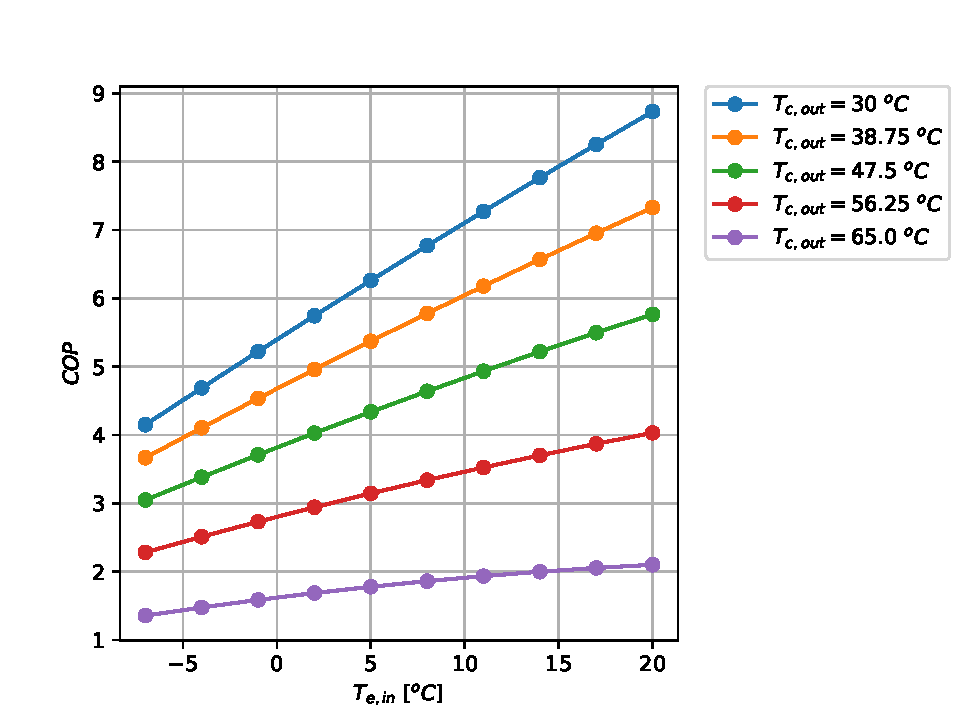
\includegraphics[width=1\textwidth]{C:/Daten/spfPackages/GIT/spfTrnsysFiles/HeatPump/BrineToWater/Walter Meier/SIN-14TU/SIN-14TU-Cop.pdf}
\caption{COP Results for the heat pump at the selected points}
\label{COPFig}
\end{center}
\end{figure}
\begin{figure}[!ht]
\begin{center}
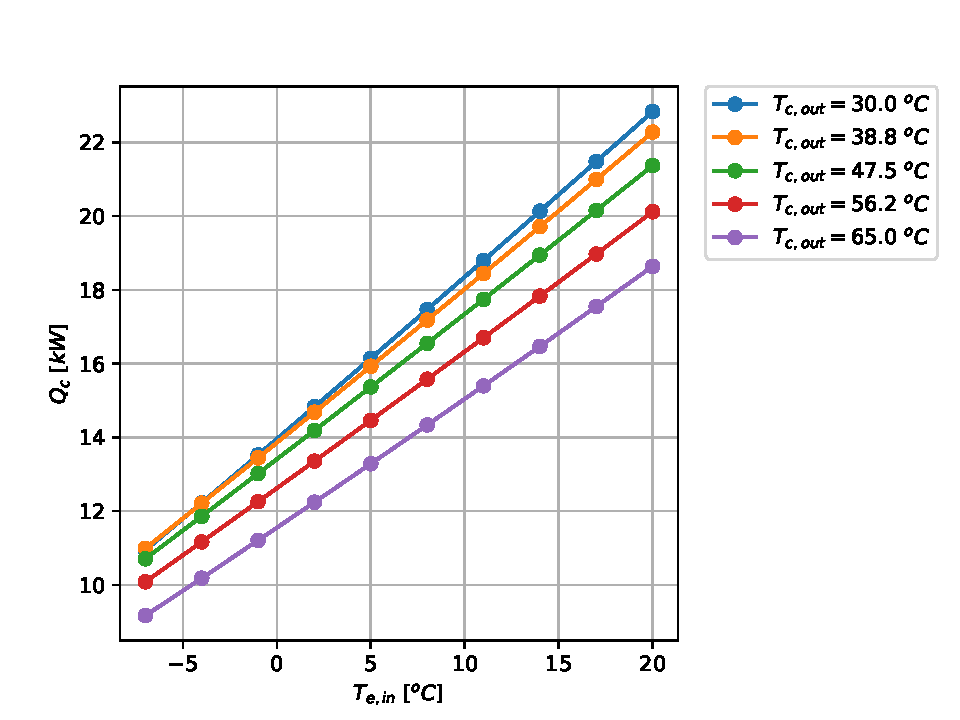
\includegraphics[width=1\textwidth]{C:/Daten/spfPackages/GIT/spfTrnsysFiles/HeatPump/BrineToWater/Walter Meier/SIN-14TU/SIN-14TU-Qc.pdf}
\caption{$Q_c$ Results for the heat pump at the selected points}
\label{QcFig}
\end{center}
\end{figure}
\end{document}
